\section{Alterations and Improvements}\label{sec:improvements}
\subsection{Improved redundancy checks}
\subsubsection{Taking advantage of data's uncertainty}\label{sec:uncertainty} 
It is not uncommon that the coefficients and right-hand-sides in the considered (in)equality system comes from approximations and/or predictions of certain circumstances, and hence the exact vertices of the feasible area is not given with high accuracy. We will therefore allow slight discrepancies between the corners of the final solution space given by our algorithm and the actual projection. 
When calculating the maximum in line~\ref{line:maxx} in Algorithm~\ref{alg:RedRem} we will therefore allow the maximum to be within a given relative $\epsilon$. That is, the condition in line~\ref{line:maxx} is replaced with the following:
\begin{equation}\label{eq:almostRed}
\max\set{\vea(c)\cdot\ve{r}}{\ve{r}\in \feas(S\setminus\{c\})}\leq \rhs(c) + \epsilon\cdot |\rhs(c)|.
\end{equation}
Though, if $\rhs(c)=0$ then we instead require the maximum to be within a certain treshold, $\epsilon'$. 

If $c$ satisfies the condition in \eqref{eq:almostRed}, we call $c$ \emph{almost redundant}, while a $c$ that satisfies the redundancy criteria in \eqref{eq:redundant} is called \emph{truly redundant}. Our definition of an almost redundant inequality is similar to the definition in \cite{lukatskii08} and \cite{shapot12}. In these paper, the authors similarly use a method for coarsening the boundary of the feasible area that relies on removing almost redundant inequalities, though it differs a bit from ours.  

\subsubsection{Concurrent redundancy checks}
The overall setup is that a manager keeps track of $k>1$ redundancy checkers to which it distributes the inequalities that need to be checked. The redundancy checkers run in parallel. Each checker starts by removing the inequalities from their own copy of the original system that the other checkers have found truly redundant so far. Then it checks if its assigned inequality is truly redundant compared to this system (see \eqref{eq:redundant} on page~\pageref{eq:redundant}) and tells the result to the manager when done. The manager then gives the idle checker a new inequality to check (if there are any left) and remembers to inform the other checkers if the examined inequality was redundant.

When using parallel redundancy checkers, it is important that we do \emph{not} remove almost redundant inequalities, i.e. inequalities that satisfy \eqref{eq:almostRed}. Otherwise, we might be in a situation as illustrated in Figure~\ref{fig:almostRedundant}, where the two inequalities $c$ and $c'$ both are almost redundant (each due to the other one). Each of them could justifiably be removed \emph{as long as} we keep the other one; removing both inequalities would result in a significantly different feasible area. Unfortunately, using parallel redundancy checkers, $c$ and $c'$ could be checked by different checkers which would then both report that their assigned inequality should be removed because it is almost redundant resulting in both inequalities being removed. Thus, we must use true redundancy for parallel redundancy checkers.
For similar reasons, when doing parallel redundancy checks it is also required that $S$ does not contain linearly dependent inequalities $c$ and $c'$ for which $\vea(c)=\sigma\cdot \vea(c')$ and $\rhs(c)=\sigma\cdot \rhs(c')$ for a positive $\sigma$, since $c$ and $c'$ in that case would define the same halfspace.

\begin{figure}[htbp]
	\centering
		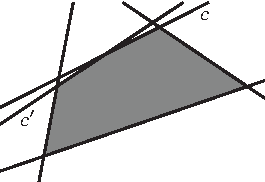
\includegraphics{figures/almostRedundant.pdf}
	\caption{Both inequalities $c$ and $c'$ are almost redundant, but only one of them can be removed from the system.}
	\label{fig:almostRedundant}
\end{figure}

However, we still let the checkers examine whether the inequalities are almost redundant (see \eqref{eq:almostRed}) and report this back to the manager who stores these. After having examined all the needed inequalities by use of parallel redundancy checkers, we then go through and check the almost redundant ones sequentially with a single redundancy checker, and remove - in turn - the ones that are still almost redundant. For the example in Figure~\ref{fig:almostRedundant} this would mean that which ever of $c$ and $c'$ is examined first is also removed, while the other is not.

The checkers also check and report on inequalities for which the optimization of its left hand side resulted in a bad condition number (also known as $\kappa$-value). This number is a measure for how much (small) differences in the input value (i.e. the coefficients and right-hand-side of the (in)equalities) effects the value of output (i.e. the found optimal value); see {e.g. \cite{numAnalysis}}. Essentially, the larger this number is, the less we can trust the result. We have chosen a threshold $\mathcal{K}$ that gives the limit for when we can trust the result. As the system gets smaller due to the removal of redundant inequalities, inequalities might be reexamined with a lower $\kappa$-value as a result, and therefore we also re-examine the inequalities that resulted in a bad $\kappa$-value when they were checked by the parallel redundancy checkers. 
Finally we also reexamine inequalities, for which the lp-solver was not able to solve the optimization of its left-hand-side.

The pseudocode for the redundancy checkers is listed in Algorithm~\ref{alg:checker}, and the pseudocode for the manager is listed in Algorithm~\ref{alg:manager}. 
When the manager receives results from the checkers (via calls to \Call{ManageResult}{} in line~\ref{line:manageResult} in Algorithm~\ref{alg:manager}), it finishes handling one call before handling the next call. 

\begin{algorithm}[htbp]
\caption{Initializing and running a redundancy checker. A checker can either check for true redundancy (used when doing concurrent redundancy checks) or not, in which case it checks for ``almost redundancy'' (for doing sequential redundancy checks).}\label{alg:checker}
\begin{algorithmic}[1]
\Function{CheckRedundancy}{Manager $m$, (In)equality system $S$, $c\in S$, boolean $\mi{truely}$}
	\State $S'\gets S$, $c'\gets c$, $\mathit{reds}\gets \emptyset$
	\While{$c' \neq $ \nul}
		\State Remove $\mi{reds}$ and $c'$ from $S'$
		\State $\mathit{max} \gets \max\set{\vea(c')\cdot\ve{r}}{\ve{r}\in \feas(S')}$
		\State Inspect solution:
		\Indent
			\State $\mathit{red}\gets \false, \mathit{recheck}\gets \false$
			\State $\kappa\gets \Call{GetConditionNumber}{\null}$
			\If{$\mathit{truely}$}
				\State $\mi{red} \gets \Call{IsTruelyRedundant?}{\mathit{max}, \rhs(c')}$ and $\kappa\leq \mathcal{K}$
				\State $\mathit{recheck} \gets \Call{IsAlmostRedundant?}{\mathit{max}, \rhs(c')}$
			\Else
				\State$\mi{red} \gets \Call{IsAlmostRedundant?}{\mathit{max}, rhs(c')}$ and $\kappa\leq\mathcal{K}$
			\EndIf
			\State $\mathit{recheck} \gets \mathit{recheck}$ or $\kappa>\mathcal{K}$ or \Call{Unsolved?}{\null}
		\EndIndent
		\If{$\neg \mathit{red}$}
			\State Add $c'$ to $S'$
		\EndIf
		\State $(c', \mi{reds})\gets m.\Call{ManageResult}{c', \mathit{red}, \mathit{recheck}}$
	\EndWhile
	\State\Return
\EndFunction
\Statex
\Function{IsTruelyRedundant?}{$\mathit{max}, \mathit{rhs}$}
	\State\Return $\mathit{max} \leq \mathit{rhs}$
\EndFunction
\Statex
\Function{IsAlmostRedundant?}{$\mathit{max}, \mathit{rhs}$}
		\State\Return ( $\mathit{rhs} = 0$ and $\mathit{max} \leq \epsilon'$) or 
				$\mathit{max} \leq \mathit{rhs} + \epsilon\cdot |\mathit{rhs}|$
\EndFunction
\end{algorithmic}
\end{algorithm}

We notice that the inequalities that should be checked for redundancy is a subset of (in)equalities in $S$. Essentially, these should be the new inequalities added to the system after each FM-elimination as described earlier. However, the function is implemented such that it is also possible to check the whole system for redundant inequalities.

\begin{algorithm}[htbp]
\caption{Managing the redundancy checkers. First a concurrent redundancy check is performed, followed by a sequential redundancy check. It is assumed that $C'$, $\mathit{reds}$ and $\mathit{rechecks}$ can be accessed by any of the manager's functions in this algorithm.}\label{alg:manager}
\begin{algorithmic}[1]
\Function{RemoveRedundancy}{System $S$, inequalities $C\subseteq S\setminus\eqs(S)$, number of checkers $k$}
	\State $S'\gets S,\; C'\gets C,\; \mathit{reds} \gets \emptyset,\; \mathit{rechecks} \gets \emptyset$, $\mi{checkers} \gets \emptyset$ 		
\State Do parallel redundancy check:
\Indent
	\DoPar{ $i\gets 1$ to $\min\{k,|C'|\}$}
		\State Add new checker $t$ to $\mi{checkers}$
		\State Call $t.\Call{CheckRedundancy}{\texttt{this}, S', \textsc{NextIneqToCheck}(), \true}$ 
	\doParUntil{all checkers in $\mi{checkers}$ have returned}
\EndIndent
\Statex
\State $S'\gets S'\setminus reds,\; C'\gets \mi{rechecks},\; \mathit{reds} \gets \emptyset,\; \mathit{rechecks} \gets \emptyset$
\State Do sequential redundancy check:
\Indent
	\If{$C'\neq \emptyset$}
		\State $t\gets $ new checker, $\mi{checkers} \gets \{t\}$ 		
		\State Call $t.\Call{CheckRedundancy}{\texttt{this}, S', \textsc{NextIneqToCheck}(), \false}$		
	\EndIf
\EndIndent
\State \Return $S'\setminus \mi{reds}$ 
\EndFunction
\Statex
\Function{NextIneqToCheck}{\null}
		\If{ $C'=\emptyset$ }
			\State\Return \nul
		\Else
			\State $c \gets$ first inequality from $C'$
			\State Remove $c$ from $C'$
			\State \Return $c$
		\EndIf
\EndFunction
\Statex
\Function{ManageResult}{Inequality $c$, boolean $red$, boolean $recheck$}\label{line:manageResult}
	\If{$red$}
		\State Add $c$ to $\mathit{reds}$
	\ElsIf{$recheck$}
			\State Add $c$ to $\mathit{rechecks}$ 
	\EndIf
	\State \Return $(\Call{NextIneqToCheck}{\null}, \mi{reds})$
\EndFunction
\end{algorithmic}		
\end{algorithm}
%
\subsection{Combining strategies}
For projecting an (in)equality system we combine the various strategies described so far in the method \Call{Project}{} presented below in Algorithm~\ref{alg:project}. It consists of steps of preprocessing the system, doing Gauss-elimination and doing FM-elimination on the system. After each FM-elimination of a variable some (timewise) ``cheap'' preprocessing steps are done, and we also make sure to remove linearly dependent (in)equalities as well. 
Hence \Call{CleanUp}{} consists of  
Algorithm~\ref{alg:prep} minus the calls to \Call{ForcedByBounds}{} and \Call{RemoveLessStrictIneqs}{}.
The reason we do not simply use \Call{Preprocess}{} is that the two above mentioned subprocedures in experience 
are more time consuming than the others and prior results showed a too little effect compared to the time taken.

After this, we remove redundant inequalities (we check only the newly added inequalities) using \Call{RemoveRedundancy}{} from Algorithm~\ref{alg:manager}. 
In \Call{RemoveRedundancy}{}, each step of doing parallel or sequential redundancy checks, respectively, are potentially repeated a number of times (or until the system does not change) depending on the values in the considered model, since ``off''-numbers (according to experience) are more likely to cause bad $\kappa$-values. If there are many inequalities resulting in bad $\kappa$-values, we would then like to test them again (after other redundant inequalities have been removed), since the removal of other inequalities can lead to a better $\kappa$-value when the inequality is re-evaluated.    
Due to the sometimes large number of inequalities that we do not know the redundancy staus of (because of a bad $\kappa$-value, that do not change during the repeated checks for redundancy), in some runs of the method we also start the FM-elimination-step in \Call{Project}{} with a full sequential redundancy check.

\begin{algorithm}\caption{Overview of the method for projecting the variables $Y$ from an (in)equality system  $S$.}\label{alg:project}
\begin{algorithmic}[1]
\Function{Project}{S,Y}
	\State $S'\gets S$
	\State $S'\gets\Call{Preprocess}{S',Y}$\Comment See Algorithm~\ref{alg:prep}
	\State $S'\gets\Call{Gauss-Elim}{S',Y}$\Comment See Algorithm~\ref{alg:Gauss} 
	\State $S'\gets \Call{FM-Elim*}{S',Y}$\Comment FM-elimination with redundancy removal (see below)
\EndFunction
\Statex
\Function{FM-Elim*}{$S,Y$}
	\State  $S'\gets S$, $Y'\gets Y$
	\While{ $Y'\neq \emptyset$ }
		\State $x\gets$ \Call{ChooseVariableToDelete}{$Y'$, $S'$}
		\State $S''\gets(\mi{Zero}_{S'}(x))_{\VAR(S')\setminus\{x\}}$
		\State $S' \gets$ \Call{FM-ElimVar}{$S'$, $x$} \Comment Algorithm~\ref{alg:FMBasic}
		\State Remove $x$ from $Y'$
		\State $S'\gets\Call{CleanUp}{S',Y}$
		\State $S'\gets \Call{RemoveRedundancy}{S', S'\setminus S'', \text{available threads}}$ 	\Comment Algorithm~\ref{alg:manager}\label{ln:projx}
	\EndWhile
	\State \Return $S'$
\EndFunction
\end{algorithmic}
\end{algorithm}
%
\subsection{Decomposition}\label{sec:decomp}
Given the theoretical complexity of the Fourier\--Motzkin\--elimination procedure, we might not have great hope of using this to eliminate a large number of variables from a very large (in)equality system, at least not if the values of the (in)equalities are randomly generated.
%
However, given an (in)equality system coming from a natural occurring problem, it is common that the constraints are \emph{block structured} \cite{williams}, where groups of constraints are ``local'' for each subdomain of the problem, while other ``global'' or ``transverse'' constraints involve many or all of the local subdomains. We will in the following assume that the given problem has a block structure and exploit this fact. 

Given a problem with block structure, the dense, ``transverse'' (in)equalities are problematic for Fourier-Motzkin-elimination, especially when they use variables that should not be eliminated, and particularly when they are equalities. 
Every time a variable in a transverse equality is eliminated, all the ``local'' (in)equalities using the variable \emph{will be combined} with one of the two inequalities corresponding to the transverse equality. The result is that we get a large number of inequalities using all the variables of the large transverse equality \emph{and} the variables from the local (in)equalities. Thus, not only do we increase the size of the problem, we also make it (much) more dense, both making the rest of the elimination process more time-consuming, and also increasing the time spend on finding redundant inequalities.
%
{Below we show how to avoid this.}
%%%%%%%%%%%%%%%%%%%%%%%%%%%%%%%%%%%%%%%%%%%%%%%%%%%%%%%%%%%%%%%%%%%%%%%%%%%%%%%%%
\subsubsection{Separating the (in)equality system}
If possible, it would be an advantage to be able to separate our (in)equality system into a (preferably large) number of smaller (in)equality systems that have ``nothing in common'', meaning that there is no overlap between the sets of variables being used in the different subsystem. If this can be done, we can then solve each subsystem separately in parallel after which the resulting systems can be combined (see Lemma~\ref{lm:projection} item \ref{lm:1.1}). As long as each subsystem is sufficiently small (such that it is can be projected in ``reasonable'' time) this may turn an insurmountable large problem into a projectable one. 
However, this is not always possible to do. Nonetheless, using the block structure to decompose the system into smaller subsystems with only little interaction by separating the system's (in)equalities can still be useful. 
 
We therefore consider $k^0$ disjoint subsets of $\VAR(S)$ - $X_1, X_2,\ldots, X_{k^0}$ - and let $X_{\texttt{t}}\odef \VAR(S)\setminus \var(\cup_{1\leq i\leq k^0}X_i)$. For each $i\in\{1,\ldots, k^0\}$ we define $S_i$ to be the (in)equality system that only uses variables in $X_i$, i.e. $S_i \odef \set{c\in S}{\var(c)\subseteq X_i}$, and we let $S_\texttt{t} = S\setminus \cup_{1\leq i \leq k_0}S_i$ be the system consisting of the rest of the (in)equalities. 

The result is that we have divided the system into $k^0$ \emph{local} parts with disjoint sets of used variables, and a \emph{transverse} part that contains (in)equalities using variables from more than one of the other local parts. 

Our (in)equality system can thus be illustrated as in Figure~\ref{fig:decomp1}.

\begin{figure}[hb]
	\centering
		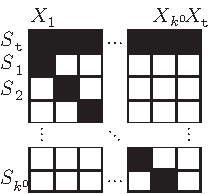
\includegraphics{figures/decomp1B2.pdf}
	\caption{Separation of the (in)equalities of an (in)equality system into local parts and a transverse part. 
	The figure shows the coefficient matrix for the system, where non-zero sections have been colored black.}
	\label{fig:decomp1}
\end{figure}

It should be noticed that in general, this can be done in many ways, but in our case - and in many common cases - there is a natural way in which the local parts/local variables present themselves. 
   
We likewise notice that for any (in)equality system, such partitions of variables and (in)equalities will always exist though they might not be very useful in practice; 
for any $X\subseteq \VAR(S)$, we can make a partition of the (in)equalities as desired, $S = \set{c\in S}{\var(c)\subseteq X}\,\dot\cup \set{c\in S}{\var(c)\not\subseteq X}$.
Intuitively, though, we have a better chance of success if $S_\texttt{t}$ is as small as possible, as well as each $S_i$ and/or $X_i$.

\begin{example}\label{ex:1}
To illustrate, let us consider the (in)equality system $S$ consisting of the following (in)equalities from which we want to eliminate all variables but $u$,  
which is defined as a sum  
of the variables $x_1, y_1, x_2, y_2, x_3, y_3$:
\begin{gather*}
\mathit{sum}: -u + x_1 + y_1 + x_2 + y_2 + x_3 + y_3= 0\\
S_1: \left\{ \begin{array}{ll}x_1 + 2 \cdot y_1 &\leq 2\\
															 -x_1 &\leq 0\\
															 -y_1 &\leq 0\end{array}\right.,\qquad
S_2 : \left\{ \begin{array}{ll} -x_2 - 3\cdot y_2 &\leq 1\\
																 x_2 &\leq 0\\
																 y_2 &\leq 0\end{array}\right.,\qquad
S_3 : \left\{ \begin{array}{ll} -x_3 + y_3 &\leq 1\\
																 2\cdot x_3 - y_3 &\leq 0\\
																 -y_3 &\leq 0\end{array}\right..
\end{gather*}
$S_1$, $S_2$ and $S_3$ are ``local'' subsystems only dealing with variables from $\{x_1,y_1\}$, $\{x_2, y_2\}$ and $\{x_3,y_3\}$, respectively. On the other hand, the equality defining $u$, 
$\mathit{sum}$, is a transverse equality. When eliminating any $x$ or $y$ variable, the system will be added (in)equalities using all variables (except the eliminated one) due to combinations with $\mi{sum}$.
\end{example}

\paragraph{Introducing auxiliary variables}
As previously mentioned it is preferable to perform elimination on a (local) subsystem such that only (in)equalities naturally ``belonging'' to that subsystem are produced, meaning that added (in)equalities uses no variables from other (local) subsystems. 
This can be achieved by the use of auxiliary variables.

Assume that $c:\sum_{x\in \VAR(c)} \coef(x,c)\cdot x \odot_c \rhs(c)$ belongs to $S_\texttt{t}$.  
For all $1\leq i \leq k^0$ we then define a variable\footnote{{Formally, we define the value of a variable in $\xx\setminus \VAR(S)$ which we will rename $z^0_{c,i}$, and so forth with all the following, defined variables}.}, $z_{c,i}^{0} \odef \sum_{x\in X_i}  \coef(x,c)\cdot x$, which can be written as an equality over $X_i\cup \{z^0_{c,i}\}$ as
\begin{equation}\label{eq:z^0_{c,i}}
\mathit{Def}(z^0_{c,i}): -z_{c,i}^{0} + \sum_{x\in X_i}  \coef(x,c)\cdot x = 0.
\end{equation}
Since $\VAR(S) = X_1 \,\dot{\cup}\; \ldots \,\dot{\cup}\; X_{k^0} \,\dot{\cup}\; X_{\texttt{t}}$ and $\coef(x,c)=0$ for $x\in \VAR(S)\setminus \var(c)$, we therefore have that 
\begin{align*}
\sum_{x\in \VAR(c)} \coef(x,c)\cdot x  
&= \sum_{x\in \VAR(S)} \coef(x,c)\cdot x \\
&= \big(\sum_{1\leq i \leq k^0}\big(\sum_{x\in X_i} \coef(x,c)\cdot x\big)\big) + \sum_{x\in X_{\ttt}}\coef(x,c)\cdot x\\
&= \big(\sum_{1\leq i\leq k^0}z^0_{c,i}\big)+\sum_{x\in X_\texttt{t}}\coef(x,c)\cdot x,
\end{align*}
which means that using the $z^0_{c,i}$-variables, $c$ can be rewritten as an (in)equality over $\cup_{1\leq i\leq k_0}\{z^0_{c,i}\}\cup X_\ttt$ as  
\begin{equation}\label{transEq}
c^0_{decp}:\big(\sum_{1\leq i \leq k^0} z_{c,i}^{0}\big) + \sum_{x\in X_\texttt{t}}\coef(x,c)\cdot x \odot_c \rhs(c).
\end{equation}
From construction it therefore follows that values for $x\in \VAR(S)$ that satisfies $c$ can be extended with values for all $z^0_{c,i}$ such that $c^0_{decp}$ and all the defining equalities (from \eqref{eq:z^0_{c,i}}) are satisfied, and vice versa, if the latter (in)equalities are all satisfied then satisfying values for the variables in $X$ will also satisfy $c$. That is,
\begin{equation}\label{eq:projz}
\feas(c)=\proj_{\cup_{1\leq i\leq k^0}\{z^0_{c,i}\}}\big(\feas(\{c^0_{decp}\}\cup\bigcup_{1\leq i\leq k^0}\{\mi{Def}(z^0_{c,i})\})\big).
\end{equation}
Using auxiliary variables for all $c\in S_\texttt{t}$ as above and adding the defining equalities $\mi{Def}(z^0_{c,i})$ to the subsystem where they belong according to their variables, we can divide the (in)equality system $S$ into a number of (in)equality systems, $S^0_1,\ldots, S^0_{k^0}, S^0_\texttt{t}$, 
as described in the pseudocode below. 

\begin{algorithm}
\caption{Separating an (in)equality system $S$ according to a list of disjoint sets of variables $\mathbb{X}=(X_1, X_2, \ldots, X_{k^0})$, where each $X_i\subseteq \VAR(S)$}\label{alg:separate}
\begin{algorithmic}[1]
\Function{SeparateIneqs}{$S$, $\mathbb{X}=(X_1, X_2, \ldots, X_{k^0})$}
\State $S_\ttt \gets \set{c\in S}{\var(c)\not\subseteq X_i\text{ for any } i}$
\For{$i\gets 1$ to $k^0$}
	\State $S^0_i \gets \set{c_{X_i}}{c\in S, \var(c)\subseteq X_i}$%\set{c_{X_i'}}{c\in S, \var(c)\subseteq X_i}$
\EndFor
\State $S^0_\ttt\gets \emptyset$ 
\ForAll{$c\in S_\ttt$}
	\For{$i\gets 1$ to $k^0$}
		\State Add $\mathit{Def}(z^0_{c,i}): -z^{0}_{c,i} + \sum_{x\in X_i} \coef(x,c)\cdot x = 0$ to $S_i^0$
	\EndFor
	\State Add $c^0_{decp}: (\sum_{1\leq i\leq k^0} z_{c,i}^0) +\sum_{x\in X_\texttt{t}}\coef(x,c)\cdot x \odot_c \rhs(c)$ to $S^0_\texttt{t}$ 
\EndFor
\State\Return ($(S^0_1,\ldots, S^0_{k^0}), S^0_\texttt{t}$)
\EndFunction
\end{algorithmic}
\end{algorithm}

The (in)equality system consisting of the union of the systems $S^0_1,\ldots, S^0_{k^0}, S^0_\texttt{t}$ will be referred to as the \emph{separated system from $S$}, written $\mi{sep}(S)$. This can be illustrated as in Figure~\ref{fig:decomp3}. For ease of notation we let $Z^0 \odef \cup_{1\leq i\leq k^0}\set{z^0_{c,i}}{c\in S_\ttt}$. We notice that for each constructed system $S^0_i$ we have that $\VAR(S^0_i)\subseteq X_i\cup Z^0$ and $\VAR(S^0_t) = X_\ttt \cup Z^0$. 

\begin{figure}[htbp]
	\centering
		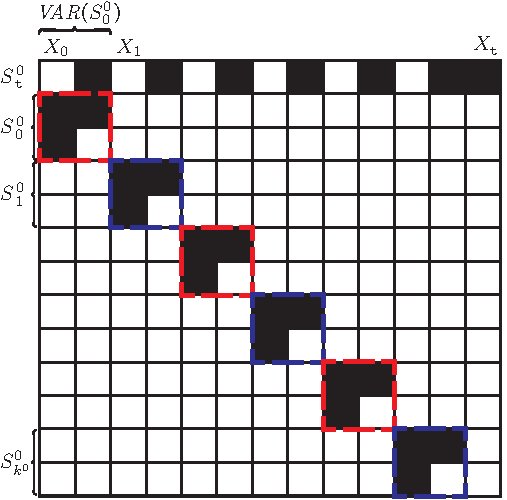
\includegraphics[scale = 0.8]{figures/decomp3B.pdf}
	\caption{The separated system from the system in Figure~\ref{fig:decomp1}. Auxiliary variables are used to prevent local constraints from different local parts to instantly ``mix'' when their variables are eliminated. Each system $S^0_i$, however, only corresponds to the system encased in coloured boxes.}
	\label{fig:decomp3}
\end{figure}

\begin{example}\label{ex:2}
Consider again the (in)equality system $S$ from Example~\ref{ex:1}. As explained, separating $S$ introduces auxiliary variables to prevent the immediate mix of variables from $\var(S_1)$, $\var(S_2)$ and $\var(S_3)$ in new inequalities when any of the variables are eliminated. This is done by defining $u$ as the sum of three auxiliary variables, $z_1$, $z_2$ and $ z_3$\footnote{For clarity of the example we do not use the variable names as described in the section above.}, which in turn are defined as the sum of the variables in each respective subsystems. Hence $\mi{sep}(S)$ is the following system.
\begin{gather*}
\mathit{sum}^0_{decp}: -u + z_1 + z_2 + z_3 = 0\\
S_1^0 : \left\{ \begin{array}{ll}-z_1 + x_1 + y_1 &= 0\\
															  x_1 + 2 \cdot y_1 &\leq 2\\
															 -x_1 &\leq 0\\
															 -y_1 &\leq 0\end{array}\right.,\qquad
S_2^0 : \left\{ \begin{array}{ll} -z_2 + x_2 + y_2 &= 0\\
																-x_2 - 3\cdot y_2 &\leq 1\\
																 x_2 &\leq 0\\
																 y_2 &\leq 0\end{array}\right.,\qquad
S_3^0 : \left\{ \begin{array}{ll} -z_3 + x_3 + y_3 &= 0\\
																 -x_3 + y_3 &\leq 1\\
																 2\cdot x_3 - y_3 &\leq 0\\
																 -y_3 &\leq 0\end{array}\right..
\end{gather*}
When we eliminate $x_1, y_1, x_2, y_2, x_3$ and $y_3$ from $S'$, we do not ``mix'' the local subsystems; this only happens when $z_1$, $z_2$ and $z_3$ afterward are eliminated. 

Furthermore, when eliminating $x_1$ and $y_1$, we only need to do this with respect to the system $S^0_1$ (and similar for $\var(S^0_2)$ and $\var(S^0_3)$). The resulting projections from $\prs_{\{x_1, y_1\}}(S^0_1)$, $\prs_{\{x_2, y_2\}}(S^0_2)$ and $\prs_{\{x_3, y_3\}}(S^0_3)$, respectively, can then be added to $\mi{sum}^0$ 
from which $z_1$, $z_2$ and $z_3$ can then be eliminated. 
%In general, this further improves the runtime of some of the subprocedures in our projection algorithm since each subsystems $S^0_1$, $S^0_2$ and $S^0_3$ will be relatively smaller than the overall system.  
\end{example}

In the end, the result is that each set $S_i^0$ now have one more (in)equality for each $c \in S_\ttt$ compared to the original $S_i$, and the number of variables in $\var(S_i^0)$ has increased with the same amount compared to $X_i$.
But, more importantly, now $|\var(S_i^0)\cap \var(S^0_\ttt)|$ equals $|S_\ttt|$, and eliminating variables in $X_i\cap Y$ will only produce (in)equalities whose set of variables is disjoint from the variable sets of the other local (in)equality systems.
Furthermore, eliminating the $z^0_{c,i}$-variables from the separated system 
will give us a system equivalent to the original system. 
Hence, eliminating the variables in $Y\subseteq \VAR(S)$ from the original system is equivalent to eliminating $Y$ and the defined $z$-variables, that is 
\[
\prs_Y(S) = \prs_{Y\cup Z^0}(\mi{sep}(S)).
\]
This follows from Lemma~\ref{lm:separating} below since by construction $\VAR(S)\setminus Y = \VAR(\mi{sep}(S))\setminus (Y\cup Z^0).$
\begin{restatable}{lemma}{separating}\label{lm:separating}
\[
\proj_Y\big(\feas(S)\big)=\proj_{Y\cup Z^0}\big(\feas(\mi{sep}(S))\big).
\]
\end{restatable}
\begin{proof}
See Appendix
\end{proof}

\subsubsection{Splitting transverse constraints}
Separating the system as described above helps preventing the (in)equalities becoming too dense when eliminating variables from the local parts. However, we also need to eliminate the defined variables in $Z^0$, which there might be many of. Using auxiliary variables in a way similar to the one described above, we would therefore like to split the variables in $Z^0$ into groups and use auxiliary variables to prevent subsystems ``mixing'' with each other. Potentially, projecting the subsystems will again result in manageable systems that can then be put together.

We will exploit the fact that if the left-hand-side of a transverse (in)equality in $S^0_\texttt{t}$ consists of a sum of many terms, it can always be rewritten as a sum of fewer terms by use of auxiliary variables. For example
\begin{align*}
z^0_{c,1} + z^0_{c,2} + \ldots + z^0_{c,k^0} &=
(z^0_{c,1} + z^0_{c,2}) + \ldots + (z^0_{c,k^0-1} + z^0_{c, k^0}) \\
&= z^1_{c,1} + \ldots + z^1_{c,k^1},
\end{align*}
where $z^1_{c,1} = z^0_{c,1} + z^0_{c,2},\; \ldots,\; z^1_{c,k^1}=z^0_{c,k^0-1} + z^0_{c,k^0}$. The latter sum can then again be rewritten into a sum of fewer terms, and so on.

\begin{example}
If we take the (separated) (in)equality system $\mi{sep}(S)$ from Example~\ref{ex:2}, the variable $u$ (which we want to keep) is now defined as a sum of three other variables ($z_1, z_2, z_3$) instead of the former six variables.  
Of course, this example is very small and a further splitting of the transverse constraints is most likely not necessary, but for the purpose of illustration, we can further split $\mi{sum}^0_{decp}$ 
such that the system obtained consists of the following (in)equalities (drawn in a tree structure)\footnote{As with Example~\ref{ex:2}, for clarity, the variable names do not follow the described naming convention.}: 

\begin{center}
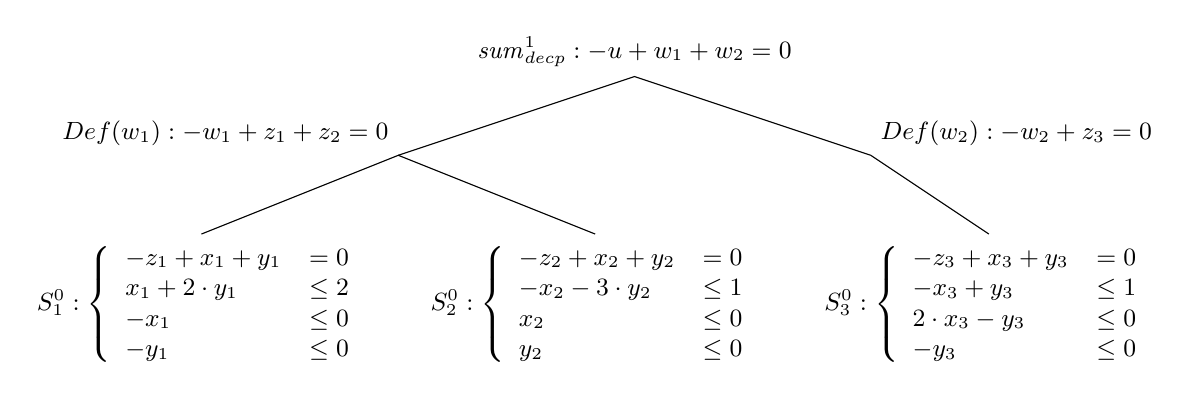
\begin{tikzpicture}
\node [above] at (6.5,3) {\small{$\mathit{sum}^1_{decp}: -u + w_1 + w_2 = 0$}};
\draw [thin] (3.5,2) -- (6.5,3) -- (9.5,2);
\node [above left] at (3.5,2) {\small{$\mi{Def}(w_1):  
																-w_1 + z_1+ z_2 = 0$}};
\draw [thin] (1,1) -- (3.5,2) -- (6,1);
\node [above right] at (9.5,2) {\small{$\mi{Def}(w_2):
															-w_2 + z_3 = 0$}};
\draw [thin] (9.5,2) -- (11,1);
\node [below] at (1,1) {\small{$S^0_1: \left\{ \begin{array}{ll}-z_1 + x_1 + y_1 &= 0\\
																x_1 + 2 \cdot y_1 &\leq 2\\
															 -x_1 &\leq 0\\
															 -y_1 &\leq 0\end{array}\right.$}};
\node [below] at (6,1) {\small{$S^0_2: \left\{ \begin{array}{ll} -z_2 + x_2 + y_2 &= 0\\
																 -x_2 - 3\cdot y_2 &\leq 1\\
																 x_2 &\leq 0\\
																 y_2 &\leq 0\end{array}\right.$}};
\node [below] at (11,1) {\small{$S^0_3: \left\{ \begin{array}{ll} -z_3 + x_3 + y_3 & = 0\\
																 -x_3 + y_3 &\leq 1\\
																 2\cdot x_3 - y_3 &\leq 0\\
																 -y_3 &\leq 0\end{array}\right.$}};
\end{tikzpicture}
\end{center}

To eliminate all variables but $u$ 
from the system, we first find projections $E^0_1\in \prs_{\{x_1, y_1\}}(S^0_1)$, $E^0_2\in \prs_{\{x_2, y_2\}}(S^0_2)$, $E^0_3\in \prs_{\{x_3, y_3\}}(S^0_3)$. Then we find projections $E^1_1\in \prs_{\{z_1,z_2\}}(E^0_1\cup E^0_2\cup  
\{\mi{Def}(w_1)\})$ and $E^1_2\in \prs_{\{z_3\}}(E^0_3\cup \{\mi{Def}(w_2)\})$ and then we find a projection $E\in \prs_{\{w_1, w_2\}}(E^1_1\cup E^1_2 \cup \{\mi{sum}^1\})$.
\end{example}
%
To further divide the transverse (in)equalities, we use an ``appropriate'' partition $\mathbb{P}^1 = (P^1_1, \ldots, P^1_{k^1})$ of the indices of the local parts, $\{1,\ldots, k^0\}$.
What is ``appropriate'' can vary, depending e.g. on the number of (in)equalities and variables in the subproblems as well as the underlying structure (if any) of the original problem.  
For each transverse (in)equality $c^0_{decp}:(\sum_{1\leq i \leq k^0}z^0_{c,i}) + \sum_{x\in X_{\texttt{t}}}\coef(x,c)\cdot x
\odot_{c}\rhs(c)$ in $S^0_\texttt{t}$ and each part $P^1_i\in \mathbb{P}^1$ we then define a variable to be the sum over the $z^0_{c,j}$-variables, whose index $j$ is in that particular part $P_i$. That is, we define the following equality $\mathit{Def}(z_{c,i}^1)$ over $\{z^1_{c,i}\}\cup\bigcup_{j\in P^i_i}\{z^0_{c,i}\}$.
\begin{equation}\label{eq:z1}
\mathit{Def}(z_{c,i}^1): -z_{c,i}^1 + \sum_{j\in P_i^1} z_{c,j}^{0} = 0.
\end{equation}
%
Using the defined variables we can then substitute in $c^0_{decp}$ to get an (in)equality over $X_\ttt\cup\bigcup_{1\leq i\leq k^1}\{z^1_{c,i}\}$.
\[
c_{decp}^1: (\sum_{1\leq i\leq k^1} z^1_{c,i}) + \sum_{x\in X_{\texttt{t}}}\coef(x,c)\cdot x \odot_c \rhs(c).
\]
Letting $Z^1 \odef \cup_{1\leq i\leq k^1}\set{z^1_{c,i}}{c\in S_\ttt}$ we can now split the newly added (in)equalities into $k^1$ ``variable-disjoint'' and one ``transverse'' (in)equality systems by defining $S^1_i\odef\set{\mi{Def}(z^1_{c,i})}{c\in S^0_\texttt{t}}$ for each $1\leq i\leq k^1$ (i.e. $\VAR(S^1_i) = \bigcup_{c\in S^0_\ttt}\VAR(\mi{Def}(z^1_{c,i}))\subseteq Z^0\cup Z^1$) and $S^1_\texttt{t} \odef \set{c_{decp}^1}{c\in S^0_\texttt{t}}$ (i.e $\VAR(S^1_\ttt) = \bigcup_{c\in S^0_\ttt}\VAR(c^1_{decp}) = X_\ttt\cup Z^1$).

If $\var(c_{decp}^1)$ is still deemed too large, i.e. $k^1$ is too large, we can repeat this step - use a partition of the indices of the previous partition to define and use auxiliary variables - until the (in)equality $c_{decp}^K$ only has a few terms, see Figure~\ref{fig:split}.

\begin{figure}
	\centering
		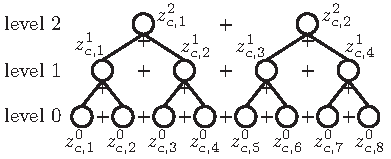
\includegraphics{figures/split.pdf}
	\caption{Splitting a transverse constraint $c^0_{decp}: \sum_{i = 1}^8 z^0_{c,i} + \sum_{x\in X_{\texttt{t}}}\coef(x,c)\cdot x\odot_c \rhs(c)$ in $S_\texttt{t}^0$ from a separated system using the partitions $\mathbb{P}^1 = \{1,2\}\;\dot\cup\{3,4\}\;\dot\cup\{5,6\}\;\dot\cup\{7,8\}$ and $\mathbb{P}^2 = \{1,2\}\;\dot\cup\{3,4\}$. 
	}
	\label{fig:split}
\end{figure}

The procedure for splitting the transverse (in)equalities like this according to a partition at a given level $l$ can be described by the following procedure \Call{SplitTransverse}{} in Algorithm~\ref{alg:split}.

\begin{algorithm}
\caption{Splitting a transverse (in)equality at the $l$'th level, according to a partition $\mathbb{P}^l$ of the indices of the previous level.}
\label{alg:split}
\begin{algorithmic}[1]
\Function{SplitTransverse}{
Transverse (in)equalities $S^0_\texttt{t}$, partitions $\mathbb{P}^l = (P^l_1, \ldots, P^l_{k^l})$}
	\State $S_\texttt{t}^l\gets \emptyset$
	\For{$i\gets 1$ to $k^l$}
		\State $S^l_i \gets \emptyset$ 
		\ForAll{$c\in S_\texttt{t}^0$}
				\State Add $\mathit{Def}(z^l_{c,i}): -z^l_{c,i} + \sum_{j\in P^l_i} z^{l-1}_{c,j} = 0$ to $S^l_i$
		\EndFor
		\State Add $c_{decp}^l: (\sum_{1\leq i\leq k^l} z^l_{c,i}) + \sum_{x\in X_{\texttt{t}}}\coef(x,c)\cdot x \odot_c \rhs(c)$
 to $S_\texttt{t}^l$
	\EndFor
	\State\Return $((S^l_1,\ldots, S^l_{k^l}), S^l_\texttt{t})$
\EndFunction
\end{algorithmic}
\end{algorithm}

At each step, we define auxiliary variables in terms of the previous level's auxiliary variables, and then we replace each decomposed transverse inequality from the previous level with another decomposed transverse inequality that uses the new auxiliary variables. The defining equalities are split into groups according to a partition of (the indices of) the previous level's variables.

Due to the definition of the new variables, $Z^l$, and the decomposed (in)equalities at the $l$'th level, it follows that eliminating the $Z^l$-variables from 
the (in)equalities defined thus far gives us an the (in)equality system consisting of all (in)equalities at the previous level; see Lemma~\ref{lm:4} below.

\begin{restatable}{lemma}{lmmmm}\label{lm:4}
\[
\proj_{Z^l}\big(\feas(S^l_\ttt\cup\bigcup_{1\leq i\leq k^l}S^l_i)\big) = \feas(S^{l-1}_\ttt)
\]
\end{restatable}
\begin{proof}
See Appendix.
\end{proof}
%
%%%%%%%%%%%%%%%%%%%%%%%%%%%%%
%%%%%%%%%%%%%%%%%%%%%%%%%%%%
%
\subsubsection*{Solving the (in)equality system exploiting structure}
Having separated the system and split the transverse (in)equalities, we can now solve the original problem, that is, eliminate the variables $Y$ from the (in)equality system $S$. The result will be an (in)equality system, whose feasible region is the projection of $Y$ from $S$, i.e. the system belongs to $\prs_Y(S)$ and will be expressed in the variables $X\setminus Y$. Though, instead of considering the whole system $S$ and eliminating the variables in $Y$ from this set, we will as previously mentioned take advantage of the decomposition of the problem. 

The overall idea of the procedure is to use the constructed decomposition of the (in)equality system to make a tree structure of subsystems where a system $S^l_i$ has the subsystems $S^{l-1}_{j}$ as a child for all $j\in P^l_i$ (see Figure~\ref{fig:treeStructureSs}). The systems corresponding to the subtrees in this structure are then projected recursively (see Figure~\ref{fig:recursiveProjectionEs} later).

{Given that the constraints of a given subproblem \emph{in real life} deals with the same aspect of the problem in question, there is a good chance that the projected subsystem with the aid of some variables significant for that aspect can be expressed in only few constraints. By separating the system and splitting the transverse constraints, which both results in divisions into subproblems, we therefore hope to better take advantage of the structure of the problem.}
\\\\
Firstly, we let $\mathfrak{S}^l_i$ denote the (in)equality system consisting of $S^l_i$ together with all it's descendants in this tree structure, see Figure~\ref{fig:treeStructureSs}. 

\begin{figure}[htbp]
	\centering
		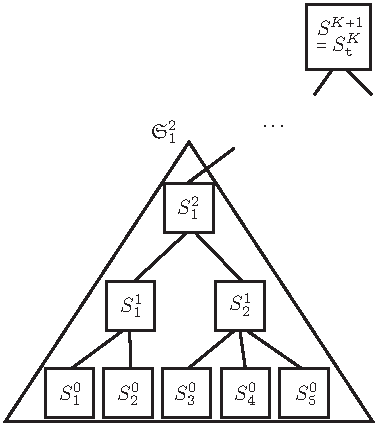
\includegraphics{figures/treeStructureSs.pdf}
	\caption{A part of the tree structure for an (in)equality system $S$. For the partitions it holds that $P^1_1, P^1_2\in \mathbb{P}^1$ where $P^1_1 = \{1,2\}$ and $P^1_2 =\{3,4,5\}$, and $P^2_1\in\mathbb{P}^2$ where $P^2_1=\{1,2\}$.}
	\label{fig:treeStructureSs}
\end{figure}

Letting $k^{K+1}=1$, $P^{K+1}_1 = \{1,\ldots, k^K\}$, and $S^{K+1}_1 = S^K_\ttt$, we formally define $\mathfrak{S}^l_i$ for all $0 \leq l \leq K+1$ and all $1\leq i \leq k^l$ as
\[
\mathfrak{S}^l_i = \left\{\begin{array}{ll}
		S^l_i \cup\bigcup_{j\in P^l_i}\mathfrak{S}^{l-1}_j&\text{if }l>0\\
		S^l_i&\text{if } l=0
\end{array}\right.
\]
Not surprisingly it is easily shown (see Lemma~\ref{lemma2} below) that $\mathfrak{S}^{K+1}$ indeed equals the union of all the defined subsystems.
\begin{restatable}{lemma}{lemmato}\label{lemma2}
\[
S^K_\ttt\cup\bigcup_{1\leq i\leq k^0}S^0_i\cup\ldots\cup\bigcup_{1\leq i\leq k^K} S^K_i = \mathfrak{S}^{K+1}_1
\]
\end{restatable}
\begin{proof}
See Appendix.
\end{proof}
%
\noindent As expected, projecting all $Y$ and $Z$-variables from the final system corresponds to projecting the $Y$ variables from the original system. From this it follows that 
\begin{equation}\label{eq:projYZ}
\prs_Y(S) = \prs_{Y\cup Z^0\cup \ldots \cup Z^K}(\mathfrak{S}^{K+1}_1)
\end{equation}
since $\VAR(S)\setminus Y = \VAR(\mathfrak{S}^{K+1}_1)\setminus(Y\cup Z^0\cup \ldots \cup Z^K)$. 
The following proposition proves the claim more formally.
\begin{restatable}{prop}{propto}\label{prop:2}
\[
\proj_Y\big(\feas(S)\big) = \proj_{Y\cup Z^0\cup \ldots \cup Z^K}\big(\feas(\mathfrak{S}^{K+1}_1)\big) 
\]
\end{restatable}
\begin{proof}
See Appendix.
\end{proof}
%
\noindent To obtain a system from $\prs_Y(S)$, we can therefore instead eliminate all $Y$ and $Z$ variables from the final system. Although this seems more troublesome, we can use the constructed tree structure to project the (in)equality system, such that a subsystem $S^l_i$ is projected by first projecting each of its subtree's systems ($\mathfrak{S}^{l-1}_j$ for $j\in P^l_i$) recursively, add these projections to $S^l_i$ and then finally project the result w.r.t. $(Y\cup Z^{l-1})\cap S^l_i$. See Figure~\ref{fig:recursiveProjectionEs}.

For each $0\leq l\leq K$ and $1\leq i \leq k^l$, we let $\mathfrak{E}^l_i$ be one of the systems in the (recursive) projection of $S^l_i$ and its subsystems (see Figure~\ref{fig:recursiveProjectionEs}). 

\begin{figure}
	\centering
		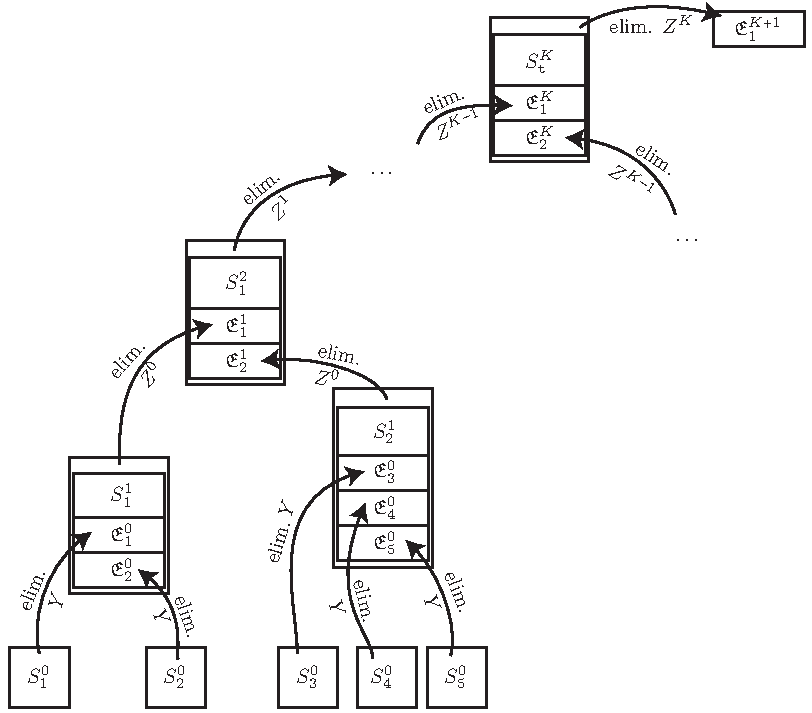
\includegraphics{figures/recursiveProjectionEs.pdf}
	\caption{Using the tree structure from Figure~\ref{fig:treeStructureSs} for an (in)equality system $S$ to recursively project the variables $Y\subseteq \VAR(S)$.}
	\label{fig:recursiveProjectionEs}
\end{figure}

\noindent More formally we define   
\begin{equation}\label{eq:mathfrakE}
\mathfrak{E}^l_i = \left\{\begin{array}{ll}
		\mathit{pick}(\prs_{Z^{l-1}}(S^l_i \cup\bigcup_{j\in P^l_i}\mathfrak{E}^{l-1}
		_j)) &\text{if }l>0\\
		\mathit{pick}(\prs_{Y}(S^l_i))&\text{if } l = 0
\end{array}\right.,
\end{equation}
where $\mathit{pick}: 2^{2^{\ie}}\to 2^{\ie}$ is an arbitrary choice-function, i.e. given a set of (in)equality systems $M$, it returns one of the (in)equality systems in $M$. As it turns out (see Lemma~\ref{lm:picking} later), the specific choice function is irrelevant for our purpose, so for now we just assume this function given.

The proposition below now gives us that projecting the $Y$- and $Z$-variables recursively as given in \eqref{eq:mathfrakE} results in the same as projecting all the variables from the final system. 

\begin{restatable}{prop}{proptre}\label{prop:3}
\[
\proj_{Z^{K}\cup \ldots \cup Z^0\cup Y}\big(\feas(\mathfrak{S}^{K+1}_1)\big) = \feas(\mathfrak{E}^{K+1}_1)
\]
\end{restatable}
\begin{proof}
See Appendix.
\end{proof}

From Proposition~\ref{prop:2} and Proposition~\ref{prop:3} it follows that $\feas(\mathfrak{E}^{K+1}_1)=\proj_Y\big(\feas(S)\big)$. It then follows from Lemma~\ref{lm:picking} below that the given choice function is irrelevant.

\begin{cor}
No matter in which way the system $\mathfrak{E}^l_i$ is chosen from $\prs_{Z^{l-1}}(S^l_i \cup\bigcup_{j\in P^l_i}\mathfrak{E}^{l-1}_j)$ (for $l>0$) or from $\prs_{Y}(S^l_i)$ (for $l=0$) we have that 
\[
\mathfrak{E}^{K+1}_1 \in \prs_{Y}(S)
\]
\end{cor}

\begin{restatable}{lemma}{picking}\label{lm:picking}
Let $p,p':2^{2^\ie}\to 2^\ie$ be such that $p(M),p'(M)\in M$ for all $M\in 2^{2^\ie}$. Then $\mathfrak{E}^l_i(p)\cong\mathfrak{E}^l_i(p')$ for all $0\leq l\leq K+1$ and all $1\leq i\leq k^l$, where
\begin{align*}
\mathfrak{E}^l_i(p) &\odef \left\{\begin{array}{ll}
		\mathit{p}\big(\prs_{Z^{l-1}}(S^l_i \cup\bigcup_{j\in P^l_i}\mathfrak{E}^{l-1}_j(p))\big) &\text{if }l>0\\
		\mathit{p}\big(\prs_{Y}(S^l_i)\big)&\text{if } l = 0
\end{array}\right.,\text{ and }\\
\mathfrak{E}^l_i(p') &\odef \left\{\begin{array}{ll}
		\mathit{p'}\big(\prs_{Z^{l-1}}(S^l_i \cup\bigcup_{j\in P^l_i}\mathfrak{E}^{l-1}_j(p'))\big) &\text{if }l>0\\
		\mathit{p'}\big(\prs_{Y}(S^l_i)\big)&\text{if } l = 0
\end{array}\right..
\end{align*}
\end{restatable}
\begin{proof}
See Appendix.
\end{proof}

\subsection{Projection framework using decomposition}
Below in Algorithm~\ref{alg:solve} we present an algorithm for finding a projection of $S$ w.r.t. $Y$ exploiting the decomposition of a block structured (in)equality system. It producing the system $\mathfrak{E}^l_i$ according to the definition in \eqref{eq:mathfrakE} for some choice-function $\mathit{pick}$. The algorithm uses a subprocedure that returns a projection of the (in)equality system $S'$ w.r.t. the set of variables $Y'\subseteq\VAR(S')$. Our framework uses \Call{Project}{} from Algorithm~\ref{alg:project} for this, but is not restricted to use this method; \Call{Solve}{} can be combined with any other method that calculates a projection in $\prs_{Y'}(S')$.

\begin{algorithm}
\caption{Projecting the variables $Y$ from an (in)equality system $S$ by decomposing it.
$\mathbb{X}=(X_1,\ldots, X_{k^0})$ is a list of disjoint subsets of $\VAR(S)$, and 
$\mathfrak{P}=(\mathbb{P}^1, \ldots, \mathbb{P}^K)$ is a list of partitions. Each $\mathbb{P}^l$ is a partition of $\{1,\ldots, k^{l-1}\}$, where $k^{i}=|\mathbb{P}^i|$ for $i>0$ and $k^0 = |\mathbb{X}|$.}
\label{alg:solve}
\begin{algorithmic}[1]
\Function{Solve}{System $S$, variables $Y\subseteq \VAR(S)$, variable sets $\mathbb{X}$, partitions $\mathfrak{P}$}
	\State $(\mathbb{S}^0,S_\texttt{t}^0) \gets \Call{SeparateIneqs}{S,\mathbb{X}}$\Comment See Algorithm~\ref{alg:separate}
	\For{$l\gets 1$ to $K$}
		\State $(\mathbb{S}^l,S^l_\texttt{t})\gets\Call{SplitTransverse}{S^0_\texttt{t},\mathbb{P}^l}$ \Comment See Algorithm~\ref{alg:split}
	\EndFor
	\State $\mathbb{S}^{K+1} =(S^K_\texttt{t})$
	\State\Return\Call{Solve-Sub}{$S^{K+1}_1, (\mathbb{S}^0, \ldots, \mathbb{S}^{K+1}), \mathfrak{P}, Y, S^0_\ttt$}
\EndFunction
\Statex
\Function{Solve-Sub}{$S^l_i, (\mathbb{S}^0, \ldots, \mathbb{S}^{K+1}), \mathfrak{P}, Y, S^0_\ttt$}
\If{$i = 0$}
	\State \Return \Call{Project}{$S^l_i$, $Y$} \label{line:project1} \Comment Algorithm¨\ref{alg:project}
\Else
	\State $S'\gets S^l_i$
	\ForAll{$j\in P^l_i$}
		\State Add \Call{Solve-Sub}{$S^{l-1}_j, (\mathbb{S}^0, \ldots, \mathbb{S}^{K+1}), \mathfrak{P}, Y, S^0_\ttt$} to $S'$ 
	\EndFor
	\State\Return \Call{Project}{$S'$, $Z^{l-1}$}\label{line:project2} \Comment Algorithm¨\ref{alg:project}
\EndIf 
\EndFunction
\end{algorithmic}
\end{algorithm}

%{We notice that in general, the order in which the variables of a given set are eliminated does not influence the final projection systems. However, there can be a (big) difference in the size of the intermediary systems that emerge after each variable elimination, both before and after redundant constraints have been removed.}
%
It should also be noted, that having the decomposition into smaller subsystems as above, it is also possible to parallelize the projection of the subproblems (either instead of or on top of the parallelization of the redundancy check). In this case, we would maintain a queue of systems, that is ready to be projected (and have not been so far), which is initialized with all leafs in the constructed tree-structure. When a system is projected, a counter for its parent is increased, and if the counter reaches the number of the node's children, it (i.e. the system with its projected child-systems) is put in the queue. Then the systems in the queue are solved independently by multiple solvers in parallel.

\subsection{Nested structure}\label{sec:nested}
The method described in Algorithm~\ref{alg:solve} first makes the separated system and thereafter splits the transverse (in)equalities. It is however possible to also use these steps in a nested fashion; on a top-level, an (in)equality system might be divided into a transverse part and a number of local parts that in themselves can be divided into further local parts and a transverse part, and so on. See Figure~\ref{fig:decompBigger}. In such a case, the presented algorithms are of course modified accordingly. 

\begin{figure}[htbp]
	\centering
		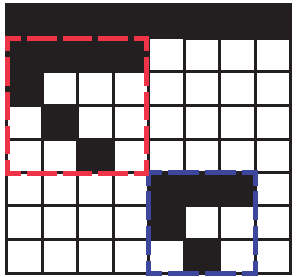
\includegraphics{figures/decompBigger.pdf}
	\caption{The inequality system in the figure can be divided into a transverse part and two local parts, namely the system enclosed within the red square and the system enclosed within the blue square. Each of the two subsystems can in themselves be solved using a decomposition into a transverse part and local parts.}
	\label{fig:decompBigger}
\end{figure}

We notice that it is up to the solver of the problem to identify the various local parts to best make use of the structure of the given problem.
However, it might be possible, also at a syntactical level, to identify potential useful partitions of the (in)equalities. This identification process is, though, left to future research. 

%\subsubsection*{\red{To be put somewhere (maybe)}}
%\red{Eliminating variables from the $X_i$ in the system consisting of all the produced constraints (and then the $z^k_{c,i}$s) will (probably) result in the same contraints being added (and being removed because of redundancy) as eliminating the $X_i$ variables from each of the smaller subproblem themselves, combining the constraints, and then eliminate the $z_i^k$-variables. The subproblems are smaller in size, so even if the two approaches adds and removes the same constraints, the latter is faster, and it is easier to keep track of which inequalities that are necessary to be taken into consideration when testing (other) inequalities for redundancy.}
%
%\red{For each defined variable $z^k_{c,i}$ there is by construction only two constraints containing it, and they would therefore be obvious choices for elimination. Though, starting with eliminating these is rather futile as we will just end with what we started with, and we could not exploit the division into subproblems.
%Hence, we solve each subproblem on its own \emph{keeping the variables} connecting them to the transverse constraints.} 
